\documentclass[10pt]{beamer}
\usetheme{Bergen}
\usepackage{caption}
\usepackage{graphicx}
\usepackage{amsmath}
\usepackage{amssymb}

\title{Van der Pol Oscillator}
\subtitle{AE 425 Project}
\institute{Indian Institute of Technology Bombay}
\date{\today}
\author{Abhilash Kulkarni}

\begin{document}

	\begin{frame}[plain]
		\maketitle
	\end{frame}

	\begin{frame}
		\frametitle{Table of Contents}
		\tableofcontents 
	\end{frame}

	\section{Introduction}
		\begin{frame}
			\frametitle{Introduction}
			The Van der Pol oscillator is a non-conservative oscillator with non-linear damping. The oscillator is defined by the following second-order differential equation:

			\begin{equation}
			\frac{d^2x}{dt^2} - \mu(1 - x^2)\frac{dx}{dt} + x = 0
			\end{equation}

			where x is the position coordinate which is a function of the time t, and μ is a scalar parameter indicating the nonlinearity and the strength of the damping.
		\end{frame}
	\section{Two-dimensional form}
		\begin{frame}
		\frametitle{Two-dimensional form}
		\textbf{Liénard's theorem\cite{wiki}} is used to prove that the van der Pol Oscillator has a limit cycle. Applying the Liénard transformation: $y = x - x^3/3 - \frac{\dot{x}}{\mu}$, the Van der Pol oscillator can be written in its two-dimensional form:
		\begin{equation}
		\dot{x} = \mu(x - \frac{1}{3}x^3 - y)
		\end{equation}
		\begin{equation}
		\dot{y} = \frac{1}{\mu}x
		\end{equation}
		Another form which is used is based on the transformation $y = \dot{x}$:
		\begin{equation}
		\dot{x} = y
		\end{equation}
		\begin{equation}
		\dot{y} = \mu(1 - x^2)y - x
		\end{equation}
		\end{frame}
\pagebreak

\begin{frame}
The system is not volume-preserving except when $\mu = 0$\cite{cornell}. If $\mu = 0$, then the equation becomes $\ddot{x} + x = 0$, the simple harmonic oscillator, which is conservative. 
\linebreak
The general van der Pol oscillator has exactly one limit cycle and all other trajectories spiral into it. All other trajectories will approach this limit cycle.
\linebreak
The following plots show the phase plot for $\mu = 0.01$ and $\mu = 2$.
\begin{figure}[h]
	\begin{tabular} {l c}
	\includegraphics[width=0.5\textwidth, height=0.5\textheight]{vanDerPol_phase_1.png} &
	\includegraphics[width=0.5\textwidth, height=0.5\textheight]{vanDerPol_phase_2.png} 
	\end{tabular}
\end{figure}
\label{fig2}

\end{frame}
\pagebreak
\begin{frame}
The first plot (for $\mu = 0.01$) shows how for low values of $\mu$ the phase plot is a circle, meaning that
the van Der Pol oscillator tends to a simple harmonic oscillator
\linebreak
\linebreak
The following plot shows the state space variables $x1 = \dot{x}$ and $x2 = \ddot{x}$ against time:

 \begin{figure}[h]
	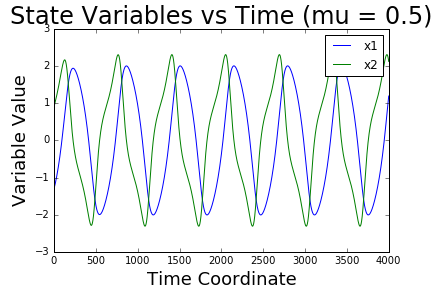
\includegraphics[width=1.0\textwidth, height=0.5\textheight]{vanDerPol_state_space.png} 
\end{figure}
\end{frame}

\bibliography{bib_file}{}
\bibliographystyle{plain}

\end{document}
